\documentclass[11pt,a4paper,]{article}
\usepackage{lmodern}

\usepackage{amssymb,amsmath}
\usepackage{ifxetex,ifluatex}
\usepackage{fixltx2e} % provides \textsubscript
\ifnum 0\ifxetex 1\fi\ifluatex 1\fi=0 % if pdftex
  \usepackage[T1]{fontenc}
  \usepackage[utf8]{inputenc}
\else % if luatex or xelatex
  \usepackage{unicode-math}
  \defaultfontfeatures{Ligatures=TeX,Scale=MatchLowercase}
\fi
% use upquote if available, for straight quotes in verbatim environments
\IfFileExists{upquote.sty}{\usepackage{upquote}}{}
% use microtype if available
\IfFileExists{microtype.sty}{%
\usepackage[]{microtype}
\UseMicrotypeSet[protrusion]{basicmath} % disable protrusion for tt fonts
}{}
\PassOptionsToPackage{hyphens}{url} % url is loaded by hyperref
\usepackage[unicode=true]{hyperref}
\hypersetup{
            pdftitle={Crime in Minneapolis},
            pdfborder={0 0 0},
            breaklinks=true}
\urlstyle{same}  % don't use monospace font for urls
\usepackage{geometry}
\geometry{a4paper, centering, text={16cm,24cm}}
\usepackage[style=authoryear-comp,]{biblatex}
\addbibresource{references.bib}
\usepackage{longtable,booktabs}
% Fix footnotes in tables (requires footnote package)
\IfFileExists{footnote.sty}{\usepackage{footnote}\makesavenoteenv{long table}}{}
\usepackage{graphicx,grffile}
\makeatletter
\def\maxwidth{\ifdim\Gin@nat@width>\linewidth\linewidth\else\Gin@nat@width\fi}
\def\maxheight{\ifdim\Gin@nat@height>\textheight\textheight\else\Gin@nat@height\fi}
\makeatother
% Scale images if necessary, so that they will not overflow the page
% margins by default, and it is still possible to overwrite the defaults
% using explicit options in \includegraphics[width, height, ...]{}
\setkeys{Gin}{width=\maxwidth,height=\maxheight,keepaspectratio}
\IfFileExists{parskip.sty}{%
\usepackage{parskip}
}{% else
\setlength{\parindent}{0pt}
\setlength{\parskip}{6pt plus 2pt minus 1pt}
}
\setlength{\emergencystretch}{3em}  % prevent overfull lines
\providecommand{\tightlist}{%
  \setlength{\itemsep}{0pt}\setlength{\parskip}{0pt}}
\setcounter{secnumdepth}{5}

% set default figure placement to htbp
\makeatletter
\def\fps@figure{htbp}
\makeatother


\title{Crime in Minneapolis}

%% MONASH STUFF

%% CAPTIONS
\RequirePackage{caption}
\DeclareCaptionStyle{italic}[justification=centering]
 {labelfont={bf},textfont={it},labelsep=colon}
\captionsetup[figure]{style=italic,format=hang,singlelinecheck=true}
\captionsetup[table]{style=italic,format=hang,singlelinecheck=true}


%% FONT
\RequirePackage{bera}
\RequirePackage[charter,expert,sfscaled]{mathdesign}
\RequirePackage{fontawesome}

%% HEADERS AND FOOTERS
\RequirePackage{fancyhdr}
\pagestyle{fancy}
\rfoot{\Large\sffamily\raisebox{-0.1cm}{\textbf{\thepage}}}
\makeatletter
\lhead{\textsf{\expandafter{\@title}}}
\makeatother
\rhead{}
\cfoot{}
\setlength{\headheight}{15pt}
\renewcommand{\headrulewidth}{0.4pt}
\renewcommand{\footrulewidth}{0.4pt}
\fancypagestyle{plain}{%
\fancyhf{} % clear all header and footer fields
\fancyfoot[C]{\sffamily\thepage} % except the center
\renewcommand{\headrulewidth}{0pt}
\renewcommand{\footrulewidth}{0pt}}

%% MATHS
\RequirePackage{bm,amsmath}
\allowdisplaybreaks

%% GRAPHICS
\RequirePackage{graphicx}
\setcounter{topnumber}{2}
\setcounter{bottomnumber}{2}
\setcounter{totalnumber}{4}
\renewcommand{\topfraction}{0.85}
\renewcommand{\bottomfraction}{0.85}
\renewcommand{\textfraction}{0.15}
\renewcommand{\floatpagefraction}{0.8}


%\RequirePackage[section]{placeins}

%% SECTION TITLES


%% SECTION TITLES (NEW: Changing sections and subsections color)  
\RequirePackage[compact,sf,bf]{titlesec}
\titleformat*{\section}{\Large\sf\bfseries\color[rgb]{0.8, 0.7, 0.1 }}
\titleformat*{\subsection}{\large\sf\bfseries\color[rgb]{0.8, 0.7, 0.1 }}
\titleformat*{\subsubsection}{\sf\bfseries\color[rgb]{0.8, 0.7, 0.1 }}
\titlespacing{\section}{0pt}{2ex}{.5ex}
\titlespacing{\subsection}{0pt}{1.5ex}{0ex}
\titlespacing{\subsubsection}{0pt}{.5ex}{0ex}


%% TITLE PAGE
\def\Date{\number\day}
\def\Month{\ifcase\month\or
 January\or February\or March\or April\or May\or June\or
 July\or August\or September\or October\or November\or December\fi}
\def\Year{\number\year}

%% LINE AND PAGE BREAKING
\sloppy
\clubpenalty = 10000
\widowpenalty = 10000
\brokenpenalty = 10000
\RequirePackage{microtype}

%% PARAGRAPH BREAKS
\setlength{\parskip}{1.4ex}
\setlength{\parindent}{0em}

%% HYPERLINKS
\RequirePackage{xcolor} % Needed for links
\definecolor{darkblue}{rgb}{0,0,.6}
\RequirePackage{url}

\makeatletter
\@ifpackageloaded{hyperref}{}{\RequirePackage{hyperref}}
\makeatother
\hypersetup{
     citecolor=0 0 0,
     breaklinks=true,
     bookmarksopen=true,
     bookmarksnumbered=true,
     linkcolor=darkblue,
     urlcolor=blue,
     citecolor=darkblue,
     colorlinks=true}

\usepackage[showonlyrefs]{mathtools}
\usepackage[no-weekday]{eukdate}

%% BIBLIOGRAPHY   %------------------------------------------------------------------------------------------------

\makeatletter
\@ifpackageloaded{biblatex}{}{\usepackage[style=authoryear-comp, backend=biber, natbib=true]{biblatex}}
\makeatother
\ExecuteBibliographyOptions{bibencoding=utf8,minnames=1,maxnames=3, maxbibnames=99,dashed=false,terseinits=true,giveninits=true,uniquename=false,uniquelist=false,doi=false, isbn=false,url=true,sortcites=false}

\DeclareFieldFormat{url}{\texttt{\url{#1}}}
\DeclareFieldFormat[article]{pages}{#1}
\DeclareFieldFormat[inproceedings]{pages}{\lowercase{pp.}#1}
\DeclareFieldFormat[incollection]{pages}{\lowercase{pp.}#1}
\DeclareFieldFormat[article]{volume}{\mkbibbold{#1}}
\DeclareFieldFormat[article]{number}{\mkbibparens{#1}}
\DeclareFieldFormat[article]{title}{\MakeCapital{#1}}
\DeclareFieldFormat[article]{url}{}
%\DeclareFieldFormat[book]{url}{}
%\DeclareFieldFormat[inbook]{url}{}
%\DeclareFieldFormat[incollection]{url}{}
%\DeclareFieldFormat[inproceedings]{url}{}
\DeclareFieldFormat[inproceedings]{title}{#1}
\DeclareFieldFormat{shorthandwidth}{#1}
%\DeclareFieldFormat{extrayear}{}
% No dot before number of articles
\usepackage{xpatch}
\xpatchbibmacro{volume+number+eid}{\setunit*{\adddot}}{}{}{}
% Remove In: for an article.
\renewbibmacro{in:}{%
  \ifentrytype{article}{}{%
  \printtext{\bibstring{in}\intitlepunct}}}

\AtEveryBibitem{\clearfield{month}}
\AtEveryCitekey{\clearfield{month}}

\makeatletter
\DeclareDelimFormat[cbx@textcite]{nameyeardelim}{\addspace}
\makeatother

\author{\sf\Large\textbf{ Lulu Pi}\\ {\sf\large Bachelor of Accounting\\[0.5cm]} \sf\Large\textbf{ Emily Sheehan}\\ {\sf\large BCom\\[0.5cm]} \sf\Large\textbf{ Brenwin Ang}\\ {\sf\large BCom\\[0.5cm]} \sf\Large\textbf{ Chengzhi Ye}\\ {\sf\large BCom\\[0.5cm]}}

\date{\sf\Date~\Month~\Year}
\makeatletter
\lfoot{\sf Pi, Sheehan, Ang, Ye: \@date}
\makeatother


%%%% PAGE STYLE FOR FRONT PAGE OF REPORTS    %----------------------------------------------------------------------------------------

\makeatletter
\def\organization#1{\gdef\@organization{#1}}
\def\telephone#1{\gdef\@telephone{#1}}
\def\email#1{\gdef\@email{#1}}
\makeatother
  \organization{Monash University}

  \def\name{Faculty of \newline Business \&\newline Economics}

  \telephone{(03) 9905 2478}

  \email{questions@company.com}                 %NEW: New email addresss ---------------------------------------

\def\webaddress{\url{http://company.com/stats/consulting/}} %NEW: URl  ------------------------------------------
\def\abn{12 377 614 630}                                    % NEW: ABN -------------------------------------------  
\def\logo{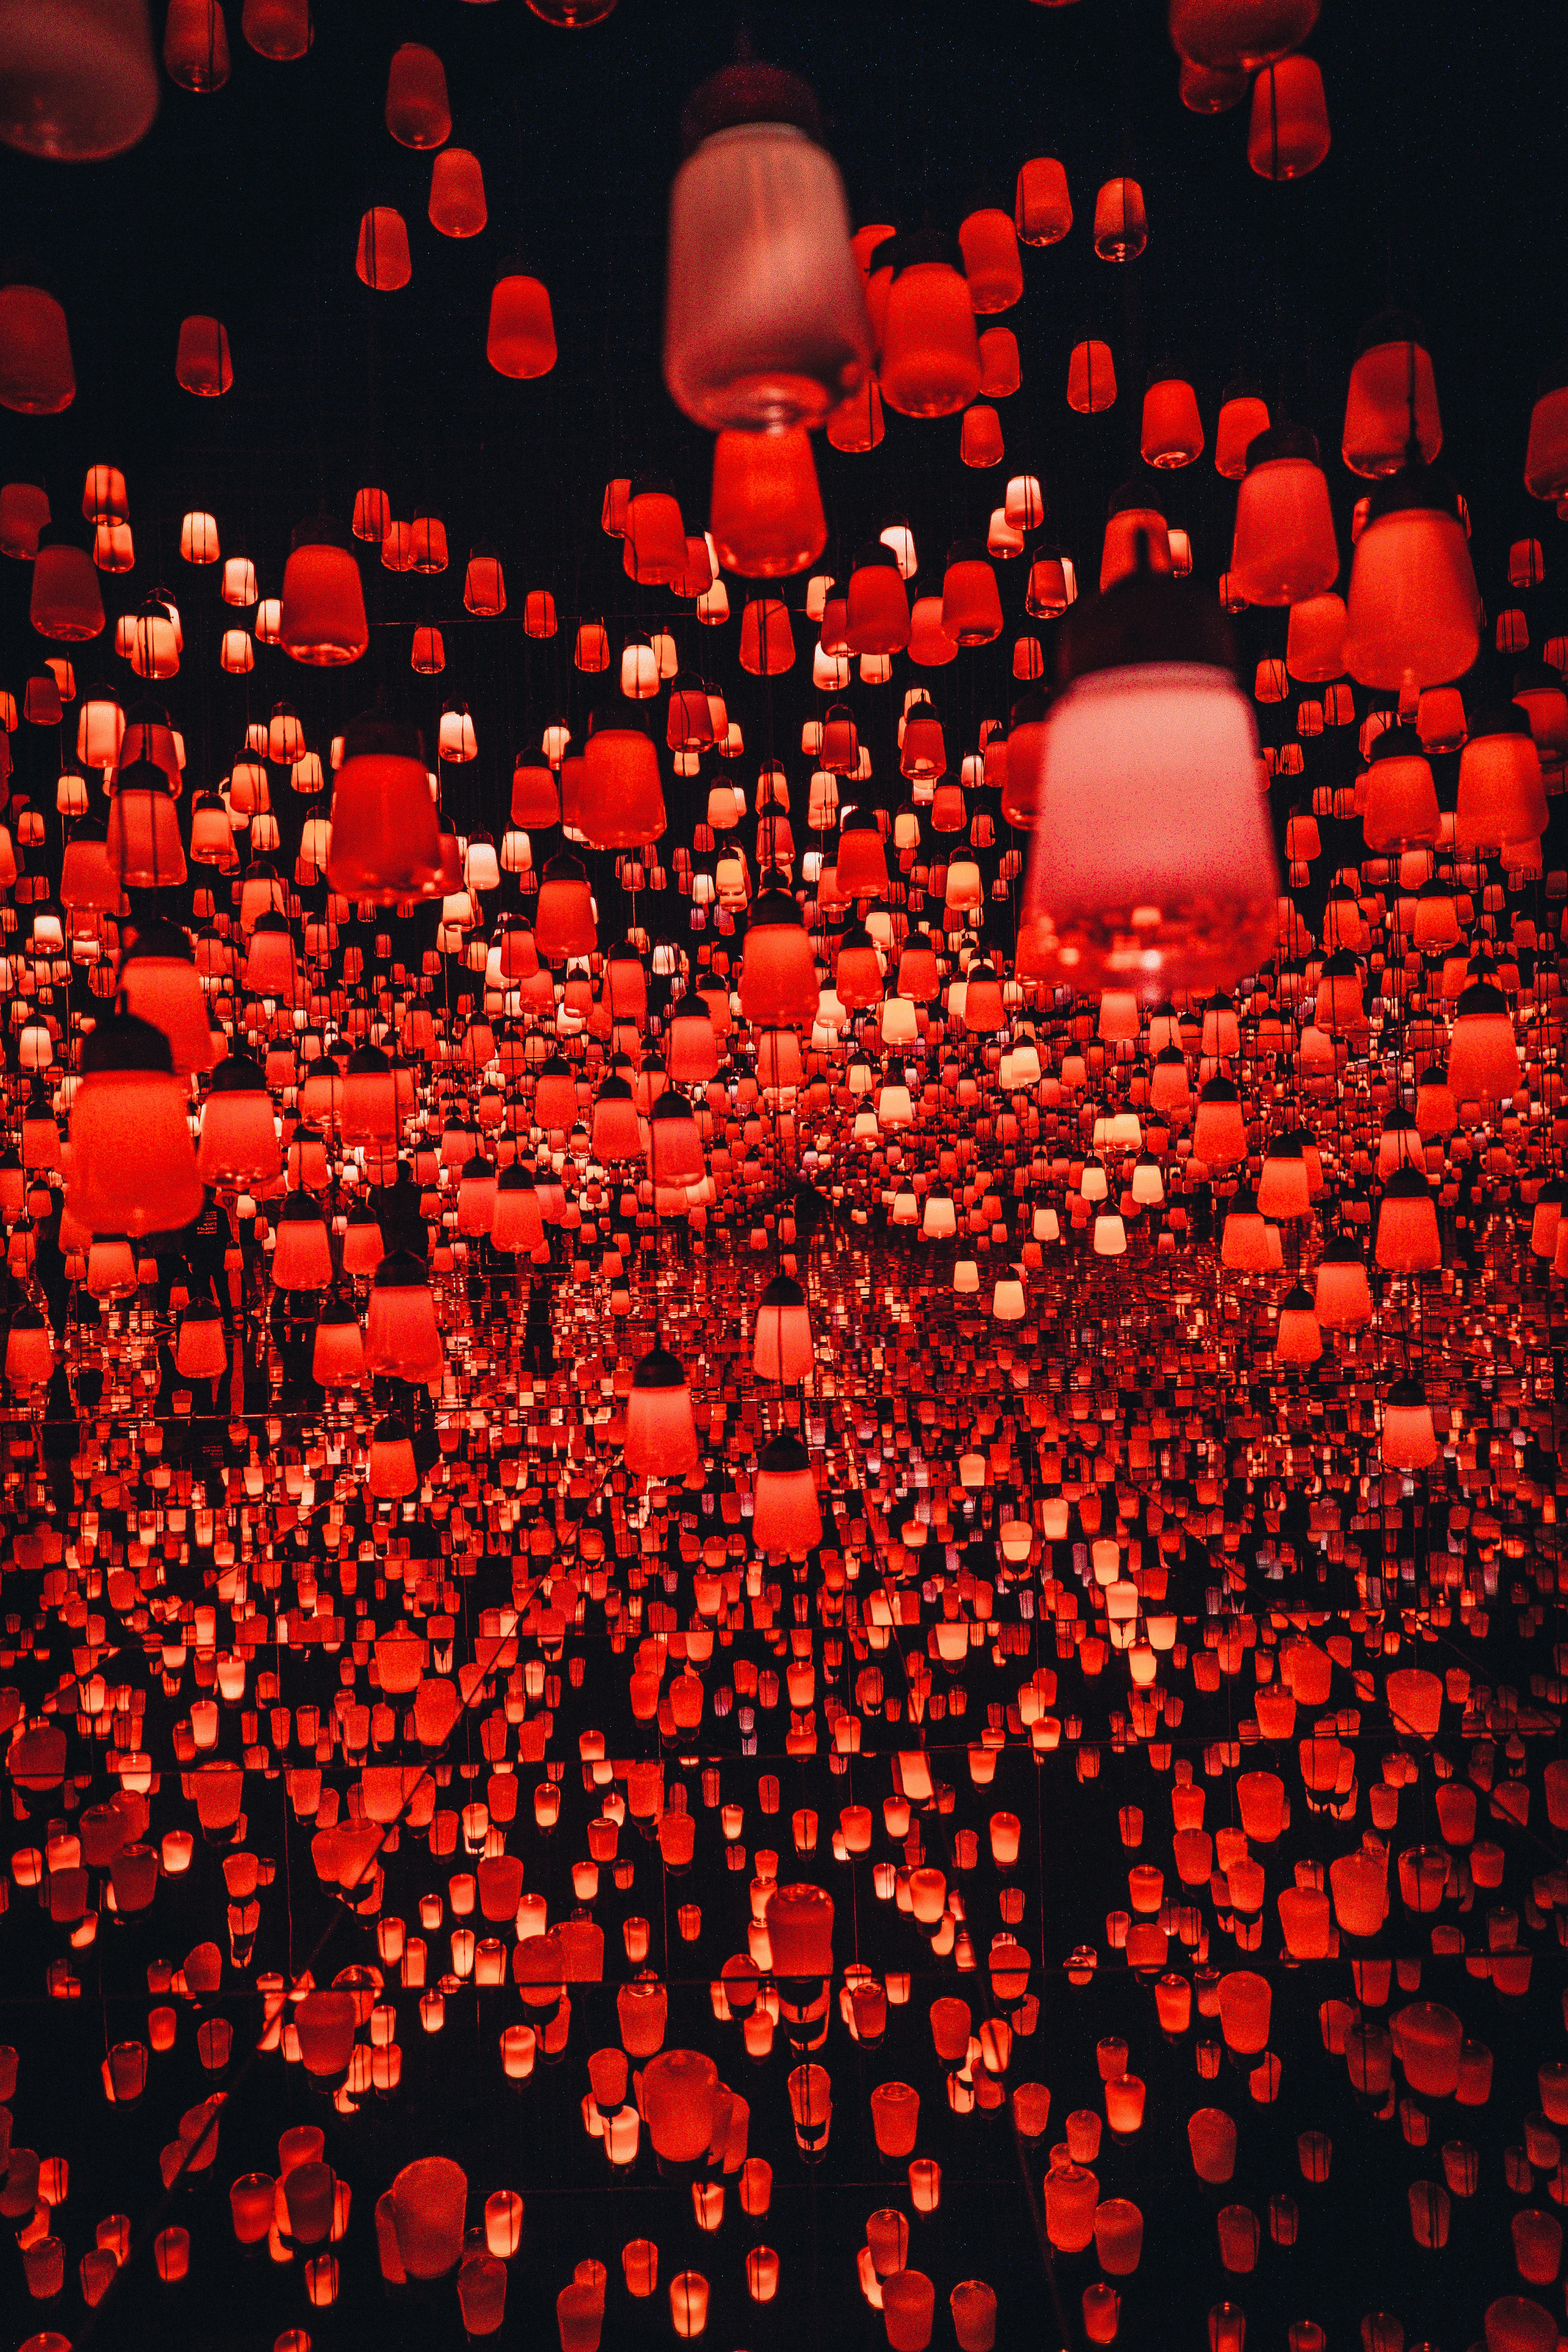
\includegraphics[width=6cm]{logo}}  %NEW: Changing logo
\def\extraspace{\vspace*{1.6cm}}
\makeatletter
\def\contactdetails{\faicon{phone} & \@telephone \\
                    \faicon{envelope} & \@email}
\makeatother

%%%% FRONT PAGE OF REPORTS

\def\reporttype{Report for}

\long\def\front#1#2#3{
\newpage
\begin{singlespacing}
\thispagestyle{empty}
\vspace*{-1.4cm}
\hspace*{-1.4cm}
\hbox to 16cm{
  \hbox to 6.5cm{\vbox to 14cm{\vbox to 25cm{
    \logo
    \vfill
    \parbox{6.3cm}{\raggedright
      \sf\color[rgb]{0, 0.29, 0.55}    % NEW color -company info------------------------------------------------------------------------------------
      {\large\textbf{\name}}\par
      \vspace{.7cm}
      \tabcolsep=0.12cm\sf\small
      \begin{tabular}{@{}ll@{}}\contactdetails
      \end{tabular}
      \vspace*{0.3cm}\par
      ABN: \abn\par
    }
  }\vss}\hss}
  \hspace*{0.2cm}
  \hbox to 1cm{\vbox to 14cm{\rule{4pt}{26.8cm}\vss}\hss\hfill}  %NEW: Thicker vertical line -----------------------------------------------------
  \hbox to 10cm{\vbox to 14cm{\vbox to 25cm{   
      \vspace*{3cm}\sf\raggedright
      \parbox{11cm}{\sf\raggedright\baselineskip=1.2cm
         \fontsize{24.88}{30}\color[rgb]{0, 0.29, 0.55}\sf\textbf{#1}}   % NEW: title color blue ----------------------------------------------
      \par
      \vfill
      \large
      \vbox{\parskip=0.8cm #2}\par
      \vspace*{2cm}\par
      \reporttype\\[0.3cm]
      \hbox{#3}%\\[2cm]\
      \vspace*{1cm}
      {\large\sf\textbf{\Date~\Month~\Year}}
   }\vss}
  }}
\end{singlespacing}
\newpage
}

\makeatletter
\def\titlepage{\front{\expandafter{\@title}}{\@author}{\@organization}}
\makeatother

\usepackage{setspace}
\setstretch{1.5}

%% Any special functions or other packages can be loaded here.


\begin{document}           % Begining of document body -----------------------------------------------
\titlepage

{
\setcounter{tocdepth}{2}
\tableofcontents
}
\clearpage

\hypertarget{introduction}{%
\section{Introduction}\label{introduction}}

George Floyd was arrested and killed by Derek Chauvin, a U.S. police officer, on the 25th of May in Minneapolis, \textcite{BBC-News-2020}. Chauvin knelt on George Floyd's neck for eight minutes and 46 seconds as Floyd gasped for air. His abominable death has sparked outrage on police brutality across America.

For several years, African-Americans have been the subject of racial vilification. In a study by \textcite{Dottolo-2008} students were interviewed and asked about police harassment and crime. Close analysis revealed that the students had stereotyped the criminals to be poor African American men.

This paper hopes to explore and understand crime in Minneapolis. Specifically, the crime incidence, the neighborhoods where crime is most common, the crime incidence over time, the force used by police and the areas where police have used force.

\hypertarget{data}{%
\section{Data}\label{data}}

To perform this analysis data was downloaded from the City of \textcite{Minneapolis-2020}. The data obtained included the shapefiles, the crime dashboard (crime incident data) and the use of force dashboard (the use of force data).

The crime incident data had a high number of missing values, where the race of the offender was not recorded. To mitigate the impact on the calculated proportions, particularly where race is concerned, they were not removed. This considered, the analysis will be impacted and the resulting proportions may be under-estimated as a result of the missing values.

The use of force data has a high number of missing values which will adversely impact the accuracy of the analysis. In addition, there is a Precinct 0 and there is no explanation on the official Minneapolis website which will certainly impact the results. The `ResponseDate' can be traced back to 2008, however, no records have been kept, therefore it cannot be used in analysis. Finally, the `PoliceUseOfForceID' and `OBJECTID' cannot be used for analysis as they are arranged in order and are independent of `real' police officers and `real' witnesses. While it protects the privacy of these individuals, it means that conclusions on aggressive police officers cannot be drawn.

\clearpage

\hypertarget{methodology}{%
\section{Methodology}\label{methodology}}

\hypertarget{analysing-the-crime-incidence}{%
\subsection{Analysing the Crime Incidence}\label{analysing-the-crime-incidence}}

The crime incident data was wrangled, and each offense was assigned to its relevant offense type. Each offense was grouped according to year, and the incidence of each offense was calculated. The results were plotted in Figure \ref{fig:plot-number-crimes}.

\hypertarget{analysing-the-neighborhoods-with-the-most-crime}{%
\subsection{Analysing the Neighborhoods with the Most Crime}\label{analysing-the-neighborhoods-with-the-most-crime}}

To create Figure \ref{fig:offencetype}, the top ten neighborhoods with the highest crime rate were plotted, and then filled according to offense.

To create Figure \ref{fig:neighborhood2018}, Figure \ref{fig:neighborhood2019} and Figure \ref{fig:neighborhood2020}, the crime incident data was cleaned, using lubridate package. It was filtered for year and grouped by neighborhood. The incidence was counted, and the top 20 neighborhoods were plotted and tabulated for each year.

For Figure \ref{fig:Crimeanalysis}, all precincts were plotted and filled according to offense.

\hypertarget{analysing-the-crime-over-time}{%
\subsection{Analysing the Crime over Time}\label{analysing-the-crime-over-time}}

The crime incident data was filtered and grouped according to year, and crime was counted for each month. The results were plotted in Figure \ref{fig:timefig}.

\hypertarget{analysing-the-force-used-by-police}{%
\subsection{Analysing the Force Used by Police}\label{analysing-the-force-used-by-police}}

To create Figure \ref{fig:weekdaysituation}, incidence for crime and force used was counted according to weekday.

The use of force data was filtered for type of resistance. The results were plotted in Figure \ref{fig:TypeOfResistance}. Each resistance band was filled according to Precinct.

To create Figure \ref{fig:relationshipfig} the use of force data was filtered for type of resistance. The results were plotted and each force type band was filled according to resistance type.

The use of force data was filtered for race. The results were plotted in Figure \ref{fig:Race} and each force type band was filled according to race.

\hypertarget{mapping-the-data}{%
\subsection{Mapping the Data}\label{mapping-the-data}}

The shape files were downloaded from Open Minneapolis, an open data repository containing spatial geographic information on Minneapolis. The shape files were used to map the neighbourhood outlines, plot the police use of force and stop data circle points, \textcite{neighbourhood}.

The data was wrangled and joined with the demographics information retrieved from \textcite{mncompass}. The information included estimates of the 5-year average neighbourhood population, collected in the 2014-2018 American Community survey. The estimates were adjusted according to the Census neighbourhood boundaries, which means that each neighbourhood could be filled according to the proportion of African Americans residing there.

\clearpage

\hypertarget{results}{%
\section{Results}\label{results}}

\hypertarget{crime-incidence}{%
\subsection{Crime Incidence}\label{crime-incidence}}

Figure \ref{fig:plot-number-crimes} demonstrates that across all years, theft is the most commonly committed crime in Minneapolis. Burglary and assault are the second and third highest committed crimes, respectively. It should be noted that 2019 is the only complete year, hence the higher incidence.

\begin{figure}
\centering
\includegraphics{Assignment4_files/figure-latex/plot-number-crimes-1.pdf}
\caption{\label{fig:plot-number-crimes}Crime incidence according to Year and Offense Type}
\end{figure}

\hypertarget{neighborhoods-with-the-most-crimes}{%
\subsection{Neighborhoods with the Most Crimes}\label{neighborhoods-with-the-most-crimes}}

Figure \ref{fig:offencetype} captures the top five most frequently committed offenses in the neighborhoods with the highest crime rates. It is clear that theft is the most commonly committed crime across all neighborhoods, consistent with Figure \ref{fig:plot-number-crimes}. Comparatively, Longflow has a similar incidence of shoplifting and theft.

\begin{figure}

{\centering \includegraphics{Assignment4_files/figure-latex/offencetype-1} 

}

\caption{The most common offence type in the Neighborhoods with the highest Crime Incidence}\label{fig:offencetype}
\end{figure}

\begin{table}

\caption{\label{tab:neighborhood-2018-table}Top 20 Neighborhoods with the Highest Crime Rate for 2018}
\centering
\begin{tabular}[t]{l|r}
\hline
neighborhood & case\\
\hline
CARAG & 194\\
\hline
Cedar Riverside & 225\\
\hline
Downtown West & 1199\\
\hline
East Phillips & 250\\
\hline
Elliot Park & 251\\
\hline
Folwell & 191\\
\hline
Hawthorne & 310\\
\hline
Jordan & 305\\
\hline
Longfellow & 378\\
\hline
Loring Park & 254\\
\hline
Lowry Hill East & 381\\
\hline
Marcy Holmes & 398\\
\hline
Near - North & 254\\
\hline
North Loop & 235\\
\hline
Powderhorn Park & 227\\
\hline
Prospect Park - East River Road & 246\\
\hline
Seward & 274\\
\hline
Ventura Village & 259\\
\hline
Whittier & 490\\
\hline
Willard - Hay & 221\\
\hline
\end{tabular}
\end{table}

\begin{table}

\caption{\label{tab:neighborhood-2019-table}Top 20 Neighborhoods with the Highest Crime Rate for 2019}
\centering
\begin{tabular}[t]{l|r}
\hline
neighborhood & case\\
\hline
Cedar Riverside & 398\\
\hline
Downtown West & 2612\\
\hline
East Phillips & 439\\
\hline
Elliot Park & 508\\
\hline
Folwell & 363\\
\hline
Hawthorne & 578\\
\hline
Jordan & 483\\
\hline
Longfellow & 768\\
\hline
Loring Park & 515\\
\hline
Lowry Hill East & 817\\
\hline
Marcy Holmes & 726\\
\hline
Midtown Phillips & 490\\
\hline
Near - North & 506\\
\hline
North Loop & 470\\
\hline
Powderhorn Park & 460\\
\hline
Prospect Park - East River Road & 414\\
\hline
Seward & 553\\
\hline
Ventura Village & 516\\
\hline
Whittier & 1182\\
\hline
Willard - Hay & 369\\
\hline
\end{tabular}
\end{table}

\begin{table}

\caption{\label{tab:neighborhood-2020-table}Top 20 Neighborhoods with the Highest Crime Rate for 2020}
\centering
\begin{tabular}[t]{l|r}
\hline
neighborhood & case\\
\hline
CARAG & 139\\
\hline
Cedar Riverside & 140\\
\hline
Downtown West & 589\\
\hline
East Phillips & 185\\
\hline
Elliot Park & 159\\
\hline
Hawthorne & 177\\
\hline
Jordan & 200\\
\hline
Longfellow & 274\\
\hline
Loring Park & 209\\
\hline
Lowry Hill East & 268\\
\hline
Marcy Holmes & 271\\
\hline
Midtown Phillips & 174\\
\hline
Near - North & 215\\
\hline
North Loop & 195\\
\hline
Powderhorn Park & 155\\
\hline
Prospect Park - East River Road & 150\\
\hline
Seward & 216\\
\hline
Ventura Village & 237\\
\hline
Whittier & 415\\
\hline
Willard - Hay & 146\\
\hline
\end{tabular}
\end{table}

\begin{figure}
\centering
\includegraphics{Assignment4_files/figure-latex/neighborhood2018-1.pdf}
\caption{\label{fig:neighborhood2018}Top 20 Neighborhoods with the Highest Crime Rate for 2018}
\end{figure}

\begin{figure}
\centering
\includegraphics{Assignment4_files/figure-latex/neighborhood2019-1.pdf}
\caption{\label{fig:neighborhood2019}Top 20 Neighborhoods with the Highest Crime Rate for 2019}
\end{figure}

\begin{figure}
\centering
\includegraphics{Assignment4_files/figure-latex/neighborhood2020-1.pdf}
\caption{\label{fig:neighborhood2020}Top 20 Neighborhoods with the Highest Crime Rate for 2020}
\end{figure}

Figure \ref{fig:neighborhood2018}, Figure \ref{fig:neighborhood2019} and Figure \ref{fig:neighborhood2020}, show that across all years \textbf{Downtown West} and \textbf{Whittier} have the highest crime rate, followed by \textbf{Longfellow}, \textbf{Lowry Hill East} and \textbf{Marcy Holmes}.

Figure \ref{fig:Crimeanalysis} explores the relationship between precinct and offense type. Across all precincts, theft is the most commonly committed crime, consistent with Figure \ref{fig:plot-number-crimes}. Interestingly enough, precinct 1 and 2 have a similar incidence of theft, however, precinct 5 has a much higher incidence of burglary.

\begin{figure}

{\centering \includegraphics{Assignment4_files/figure-latex/Crimeanalysis-1} 

}

\caption{Crimes comparison of different districts}\label{fig:Crimeanalysis}
\end{figure}

\hypertarget{crime-over-time}{%
\subsection{Crime over Time}\label{crime-over-time}}

Figure \ref{fig:timefig} compares the incidence of crimes in each month. As stated above, 2019 is the only complete year in the data set. In 2018, crime peaked in October, and dropped in December. In 2019, crime was very low in the colder months (January, February and March), peaking in the summer months (July and August). Comparatively, the incidence of crime in 2020 was much lower than 2019 and did not increase in May, which is likely due to the stay at home orders resulting from COVID-19.

\begin{figure}

{\centering \includegraphics{Assignment4_files/figure-latex/timefig-1} 

}

\caption{Comparison of crimes in different months}\label{fig:timefig}
\end{figure}

\hypertarget{force-used-by-police-data}{%
\subsection{Force Used by Police Data}\label{force-used-by-police-data}}

Figure \ref{fig:weekdaysituation} shows the distribution of the total crimes and force used over the week. There are more crimes on weekdays than on weekends, however, there is greater force use on weekends. It is likely that entertainment venues draw large crowds on the weekends, therefore attracting a large police presence. Furthermore, it is unlikely criminals will commit crimes, particularly when police presence is so high.

\begin{figure}

{\centering \includegraphics{Assignment4_files/figure-latex/weekdaysituation-1} 

}

\caption{The average crimes and force used in a given week}\label{fig:weekdaysituation}
\end{figure}

Figure \ref{fig:TypeOfResistance} shows the resistance used in each precinct. In essence, this figure captures the prevalence of crime and the efficiency of police in controlling the crime rate. It can be inferred that the fourth precinct is significantly more dangerous than the fifth precinct, and the force use in the fourth precinct is much higher.

\begin{figure}

{\centering \includegraphics{Assignment4_files/figure-latex/TypeOfResistance-1} 

}

\caption{The different Resistance of criminals in each Precinct}\label{fig:TypeOfResistance}
\end{figure}

Figure \ref{fig:relationshipfig} shows the relationship between the force type and the type of resistance. This figure captures the effectiveness of the force type used by police. For example, if the only resistance used by police is a police dog, criminals are more likely to flee on foot. However, if a firearm or chemical irritant is used, better results will be achieved.

\begin{figure}

{\centering \includegraphics{Assignment4_files/figure-latex/relationshipfig-1} 

}

\caption{The relationship between Force Type adopted by police and type of resistance of criminals}\label{fig:relationshipfig}
\end{figure}

Figure \ref{fig:Race} shows the use of force on different races. African Americans are subject to more aggressive forms of force. The figure clearly demonstrates that police are less likely to use less lethal force on African Americans. Looking at this figure alone, it is likely that the treatment of African Americans is unnecessarily barbaric.

\begin{figure}

{\centering \includegraphics{Assignment4_files/figure-latex/Race-1} 

}

\caption{Different races are treated differently}\label{fig:Race}
\end{figure}

\hypertarget{mapping-the-data-1}{%
\subsection{Mapping the Data}\label{mapping-the-data-1}}

\begin{table}

\caption{\label{tab:summarytable}Proportion of African Americans for each Category}
\centering
\begin{tabular}[t]{l|r}
\hline
categories & share\\
\hline
Minneapolis Population & 0.20\\
\hline
Police Use of Force & 0.60\\
\hline
Police Stop & 0.53\\
\hline
\end{tabular}
\end{table}

African Americans count for 20\% of the total population in Minneapolis, \textcite{mncompass}. However, they are most likely to be stopped by police and the subject of police force as in table \ref{tab:summarytable}. Note that all proportions are subject to a 5\% or less margin of error.

\begin{figure}
\centering
\includegraphics{Assignment4_files/figure-latex/puofmap-1.pdf}
\caption{\label{fig:puofmap}Police use of force data on a Minneapolis Map}
\end{figure}

Figure \ref{fig:puofmap} shows Minneapolis, segmented by neighbourhoods. The shade of green represents the number of African Americans in each neighbourhood; with dark green indicating a higher proportion of African Americans. Each circle represents an incident where police used force, and the color represents the ethnicity of the subject. Minority groups were classed as `others'.

There's a high concentration of African Americans living in the north-west and centre of Minneapolis. These areas also have a high number of incidents where police have used force against African Americans.

\begin{figure}
\centering
\includegraphics{Assignment4_files/figure-latex/psbar-1.pdf}
\caption{\label{fig:psbar}Counts per Race in each reason to stop a Vehicle}
\end{figure}

Figure \ref{fig:psbar} shows the number of cars stopped for a given reason, according to race. African Americans were the most likely to be stopped for all reasons.

\begin{figure}
\includegraphics[width=4\linewidth]{Assignment4_files/figure-latex/psmap-1} \caption{Police Stop data on Minneapolis map}\label{fig:psmap}
\end{figure}

A similar pattern to Figure \ref{fig:puofmap} was observed in Figure \ref{fig:psmap}. Police stops are highly concentrated in the north western and central areas of Minneapolis, where African American communities are highly represented.

\hypertarget{conclusion}{%
\section{Conclusion}\label{conclusion}}

Theft is the most commonly committed crime in Minneapolis. Downtown West and Whittier are the neighborhoods with the highest crime rate. Interestingly enough, the crime rate tends to be lower in the colder months of the year, and has been lower in 2020 due to the stay at home orders resulting from COVID-19. The crime rate is higher during the week, while the force use is much higher on weekends; indicating a greater police presence on weekends.

Analysis of the use of force dashboard revealed that police dogs are generally ineffective in arrests as criminals are more likely to flee on foot. The use of force towards African Americans is significantly higher for all force types, except the less lethal force type. This is disproportionate to the number of African Americans in Minneapolis. Additionally, the incidence of force use on African Americans and the number of African Americans stopped is much higher in communities where African Americans are highly represented. Unfortunately, the analysis has divulged clear patterns of discrimination which is deeply distressing and calls for immediate action.

\clearpage

The following packages were used; \textcite{tidyverse}, \textcite{rgdal}, \textcite{ggrepel}, \textcite{scales}, \textcite{gridExtra}, \textcite{kableExtra}, \textcite{lubridate}, \textcite{ggpubr}, \textcite{RColorBrewer}, \textcite{leaflet}, \textcite{knitr}, \textcite{sf}.

\printbibliography

\end{document}

